\section{Klassifizierung einer Webseite}
    \label{section:conceptClassification}
    Der Spezifikation eines Klassifizierungsmodells folgt die Durchführung einer Klassifizierung,
    worüber dieses Kapitel einen allgemeinen Überblick verschafft.

    \subsection{Datenquelle}
        \label{section:conceptClassificationDataSource}
        Die erste zu klärende Frage ist, welche Repräsentation einer Webseite
        das \gls{wccs} zur Klassifizierung verwendet und woher es diese bezieht.
        Für den Fall der {\fernUni} bietet {\wordpress} zwei Schnittstellen,
        um Informationen über Beiträge und Seiten abzufragen:

        \begin{enumerate}
            \item Die Datenbanktabelle \texttt{wp\_posts} \cite{wordpress:Database}
            \item Einen RESTful Web-Service \cite{wordpress:RestAPI}
        \end{enumerate}

        Beide Quellen stellen das \gls{wccs} vor Herausforderungen.
        Die Inhalte der Datenbank verwenden neben \gls{html} zum Beispiel die speziellen
        Auszeichnungssprachen der Plugins, die in einem Beitrag genutzt werden.
        Diese müssten vom \gls{wccs} interpretiert werden,
        um die Inhalte, die diese Plugins produzieren, zu erfassen.
        Der RESTful Web-Service übernimmt diese Aufgabe und übermittelt
        eine reine \gls{html}-Repräsentation des angeforderten Beitrages,
        was ein Argument für seine Verwendung ist.

        Allerdings ist auch über diesen Dienst nur der spezielle Inhalt eines
        Posts oder einer Page zugänglich.
        Das heißt, dass Inhalte, die in Templates definiert werden, über beide
        Schnittstellen nicht bezogen werden können.
        Das betrifft zum Beispiel den Kopfbereich der Seiten der Fakultät \gls{ksw}.
        Ob dies ein gravierendes Manko ist, hängt unter anderem davon ab,
        ob solche allgemeinen Bereiche relevant für eine Klassifizierung sind
        und wie viele seitenspezifische Inhalte sie besitzen.
        Ein Nachteil ist allerdings, dass externe Systeme über diese Schnittstellen
        nur schwer ermitteln können, wo die Inhalte eines Beitrages auf der vollständigen Seite genau positioniert sind.
        Das erschwert dem \gls{wccs} die später beschriebene Visualisierung einer
        Klassifikation\footnote{vgl. \ref{section:conceptVisualization}}.       

        Ein weiterer zu beachtender Aspekt ist, dass diese Quellen {\wordpress}-spezifisch sind,
        wodurch das \gls{wccs} eine starke Bindung zu diesem \gls{cms} erhalten würde
        und weniger allgemein einsatzbar wäre.

        Eine Alternative, die auch sämtliche oben beschriebenen Probleme löst,
        ist die Nutzung der \gls{html}-Repräsentation einer Webseite,
        die über ihre \gls{url} bezogen wird.
        Diese verwendet eine standardisierte Sprache (\gls{html}) und enthält
        die vollständige Seite, sodass auch die im \gls{cms} global definierten Inhalte,
        wie ein Kopfbereich, leicht einer Klassifizierung unterzogen werden können.
        Gleichzeitig macht es das \gls{wccs} vollkommen unabhängig vom verwendeten \gls{cms}.

    \subsection{Allgemeiner Ablauf}
        \label{section:solutionConceptClassificationAlg}
        % TODO: erwähnen, dass mit Spezifikation konfiguriert
        Der allgemeine Ablauf der Klassifizierung lässt sich leicht und in wenigen Sätzen beschreiben.
        Da als Quelle die Live-Seite herangezogen wird, ist Eingabe die \gls{url} dieser Seite.

        Das System bestimmt zunächst die Klasse der Seite, indem die verschiedenen Selektoren der bekannten
        Seitenklassen gegen sie geprüft werden.
        Dann werden die Features dieser Klasse auf der Seite ermittelt,
        indem die Selektoren der Features auf der Seite angewandt werden.
        Für jedes Content Feature wird die Ermittlung der Features rekursiv wiederholt.
        Anschließend wird die gesamte Klassifikation persistiert.

    \subsection{Unterstützte Selektoren}
        \label{section:conceptSupportedSelectors}
        Das Klassifizierungssystem unterstützt drei Selektoren,
        die durch die gewählte Datenquelle begründet sind.
        Eine andere Quelle hätte womöglich zu anderen Selektoren geführt.

        Die Selektoren sind ein CSS-Selektor, ein XPath-Selektor und ein URL-Selektor
        und werden jetzt vorgestellt.

        % TODO: CSS wählt immer einen Knoten, Xpath Knoten oder Text

        \paragraph{CSS-Selektor}
        Der CSS-Selektor kann für Features verwendet werden und benutzt
        die durch das \gls{w3c} standardisierten CSS-Selektoren
        (siehe Kapitel \ref{section:wwwTechnicalFoundations} und \cite{w3c:cssSelectors}),
        um einen oder mehrere Nodes im \gls{html}-Dokument auszuwählen.
        Da diese Selektoren auf mehrere Nodes zutreffen können,
        sind Collection Featues direkt unterstützt.

        Das \gls{wccs} folgt bei der Auswertung eines CSS-Selektors der Logik des \glspl{w3c}
        \cite{w3c:selectorsAPI}.
        Das bedeutet, dass der Selektor für das gesamte Dokument ausgeführt,
        aber nur Elemente innerhalb des Parent Features im Ergebnis landen.
        Für Features der ersten Ebene wird document als Kontext-Node genommen.
        Dadurch ist sichergestellt, dass sich wiederholende Strukturen richtig zugeordnet werden können.

        Dazu ein Beispiel. Angenommen es gibt ein CollectionFeature mit dem CSS-Selektor
        "`article"'. Dieser wählt die drei article-Nodes aus.
        Die Klasse dieses Features hat wiederum ein Feature "`heading"' mit dem Selektor
        "`h3"'.
        Da dieser im Kontext des jeweiligen article-Nodes ausgeführt wird,
        ist klar, welche Überschrift zu welchem Artikel gehört.

        \begin{lstlisting}
<article>
    <h3>Article 1 Heading<h3>
</article>
<article>
    <h3>Article 2 Heading<h3>
</article>
<article>
    <h3>Article 3 Heading<h3>
</article>
        \end{lstlisting}

        \paragraph{XPath-Selektor}
        Der XPath-Selektor ist ebenfalls für Features geeignet und wertet auf dem
        HTML-Dokument XPath-Ausdrücke aus, um Nodes zu selektieren.
        Im Vergleich zu CSS ist XPath in manchen Belangn mächtiger.
        Zum Beispiel erlaubt es den aktuellen Node über "`self"' zu matchen,
        Siblings des aktuellen Nodes zu selektieren
        oder Nodes in anderen Teilen des Dokumentes zu selektieren \cite{w3c:xpath}.
        Ein XPath-Selektor verwendet ebenfalls document bzw. den Node des Parent Features als
        Kontext Node.
        Die über CSS-Selektoren garantierte Relativität kann vom Nutzer mit den oben genannten Mitteln
        durch XPath-Selektoren allerdings umgangen werden,
        wodurch er mehr Möglichkeiten, aber auch mehr Verantwrotung erhält.

        \paragraph{\gls{url}-Pattern-Selektor}
        Ein \gls{url}-Pattern-Selektor ist für Seiten und Referenzen geeignet.
        Bei diesem Selektor handelt es sich um einen regulären Ausdruck,
        der im Falle von Seiten auf deren \gls{url} angewandt wird.
        Gibt es ein Match, wird die Seite entsprechend klassifiziert.
        
        Zur Klassifizierung von Referenzen wird der Selektor auf die \gls{url} aller Knoten
        innerhalb des Parent Features angewandt, die eine {\resource} referenzieren.
        Gibt es ein Match, wird der Node als entsprechendes Referenz Feature erkannt.
        Da alle Nodes geprüft werden, sind Collection Features kein Problem.

        Dieser Selektor ist sinnvoll, um zum Beispiel externe Links anders als interne zu klassifizieren.

    \subsection{Datenmodell des Klassifizierungsergebnisses}
        \label{section:conceptPageDataModel}
        % TODO: Muss das ggf. höher, vllt. direkt nach Klassen, Features, Selektoren?
        % TODO: Muss der RangeSelector vielleicht doch enthalten sein?
        Dieses Kapitel beschreibt anhand Abbildung \ref{image:conceptPageDataModel}
        das Modell einer Klassifikation einer Seite.

        \begin{figure}[htb]
            \centering
            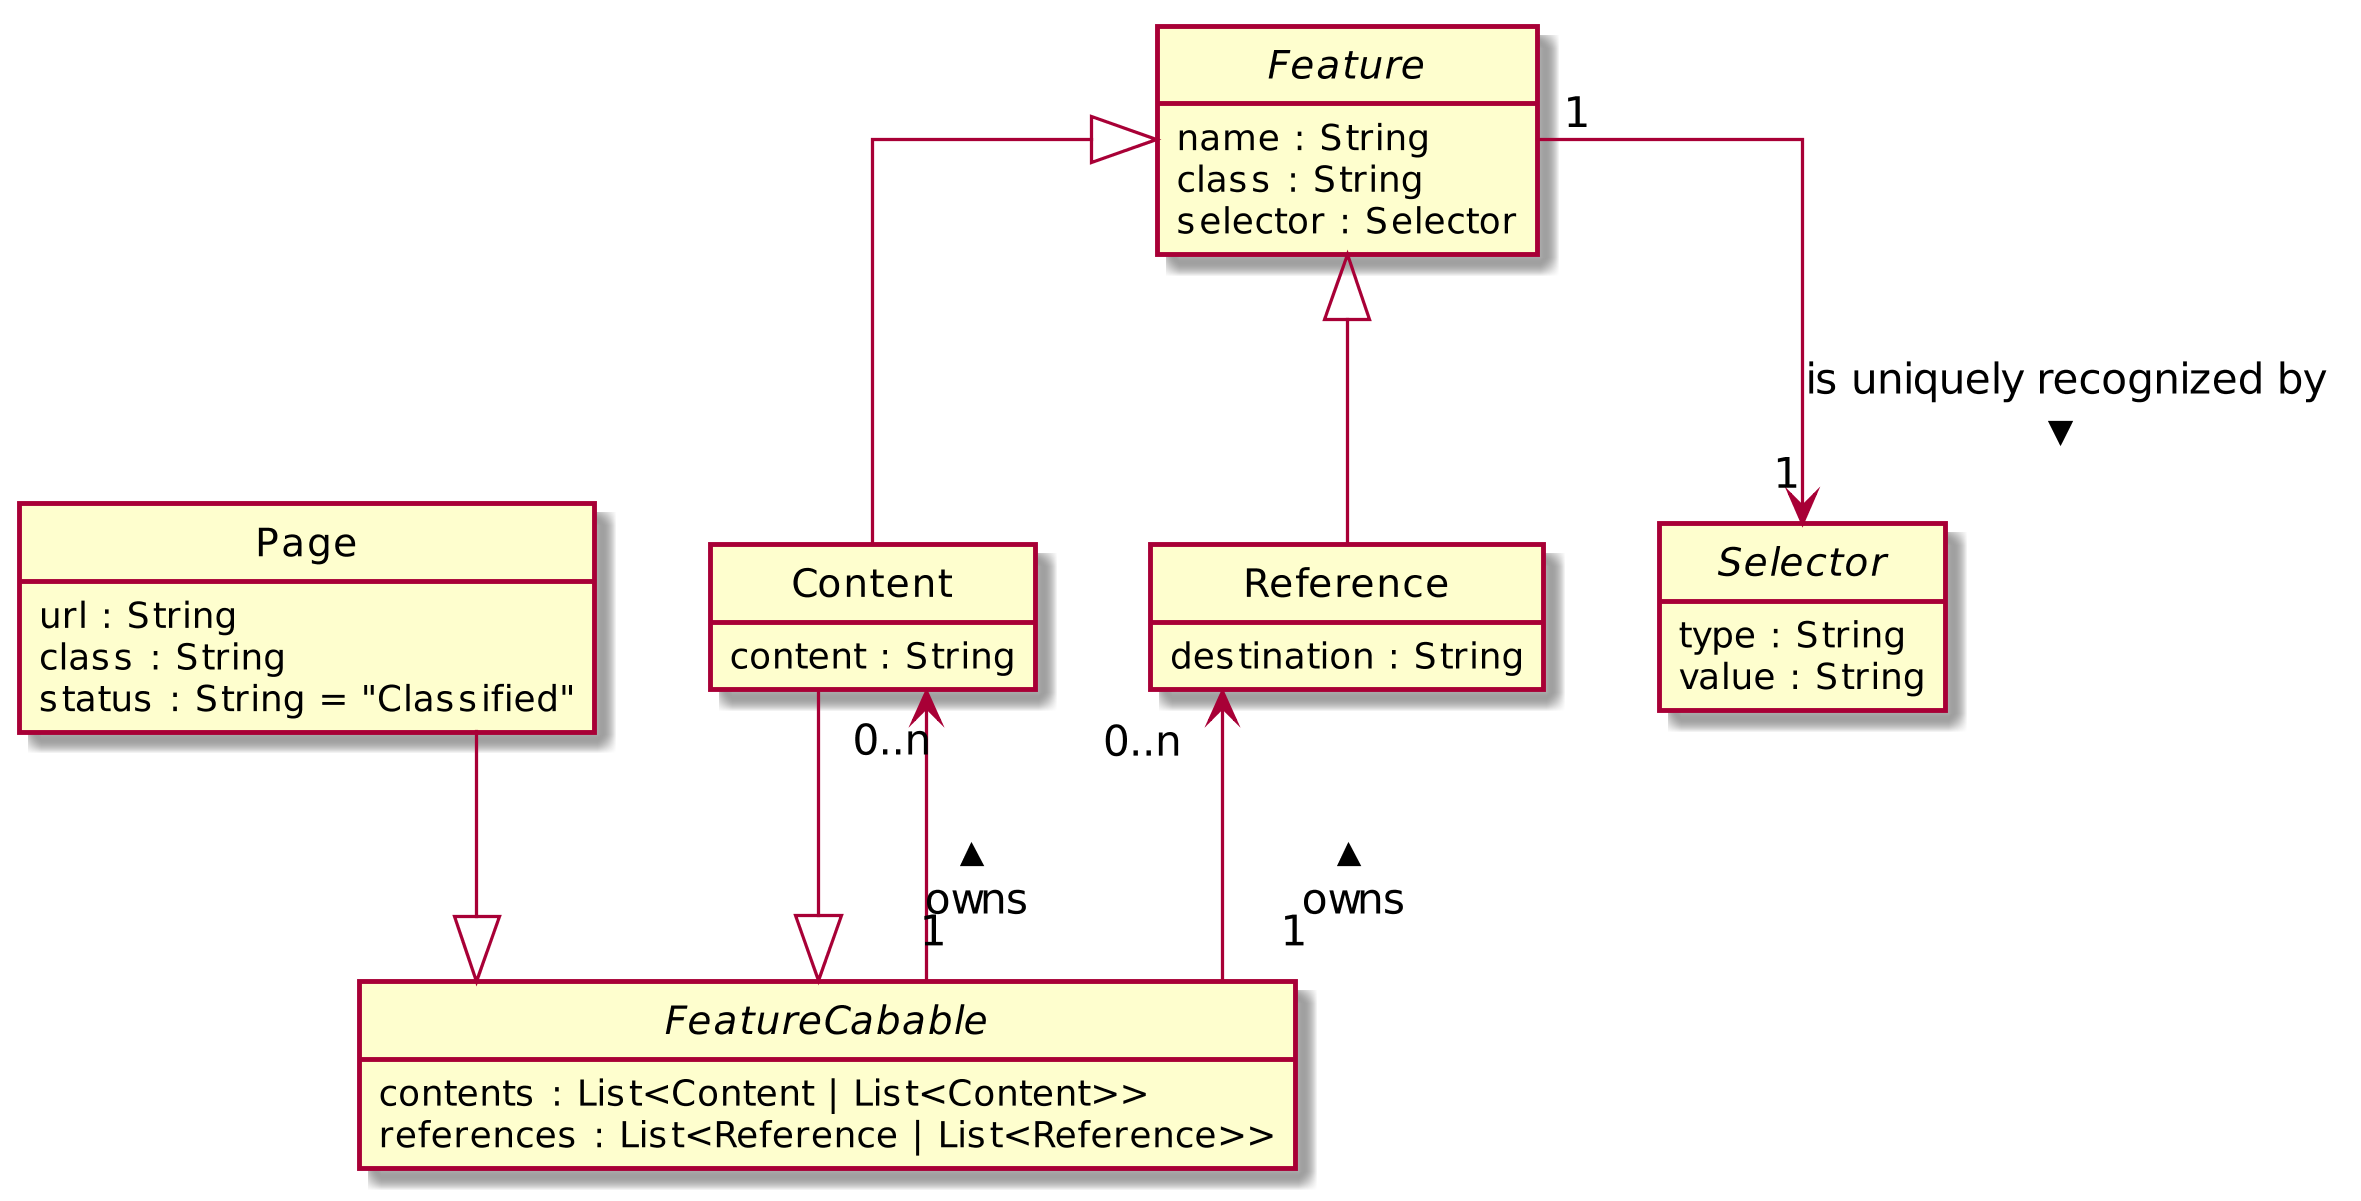
\includegraphics[scale=\imageScalingFactor]{../resources/concept/page.png}
            \caption{Datenmodell eines Klassifizierungsergebnisses}
            \label{image:conceptPageDataModel}
        \end{figure}

        Oben in der Hierarchie steht die Seite,
        zu der ihre \gls{url} und ihre Klasse gespeichert wird.
        Außerdem hat sie einen Status, der nach der Klassifizierung auf
        "`Classified"' gesetzt ist.
        Des weiteren speichert eine Seite in zwei getrennten Listen ihre
        Content- und Reference Features.
        Elemente dieser Listen können Content oder Reference Objekte oder Listen
        dieser Objekte sein. Listen spiegeln CollectionFeatures wieder.
        Jedes Feature speichert seinen Namen und seine Klasse.
        Content Features darüber hinaus ihren textuellen Inhalt % TODO WARUM?!
        und Reference Features die \gls{url} der referenzierten {\resource}.
        Features speichern außerdem einen Selektor, bei dem es sich nicht um den Selektor
        handelt, der während der Klassifizierung zu ihrer Ermittlung verwendet wurde.
        Stattdessen identifiziert dieser Selektor den zum Feature gehörenden Node eindeutig im HTML-Dokument.
        Das ist später z. B. für die Visualisierung der Klassifikation hilfreich.
        Außerdem bietet es Drittsystemen die Möglichkeit leicht festzustellen,
        ob sich der Inhalt eines Contents oder das Ziel einer Referenz seit der Klassifizierungssystem
        geändert hat.
